% Origen: Secciones/PI - Software.md
% Su sección "Apéndice" está en apend5.tex (Complementos del software).
\chapter{Software}
\label{C:sw}

% Figuras de ESTE capítulo + las compartidas. Siempre al principio del archivo.
\graphicspath{{figs/cap10/}{figs/comunes/}}

\begin{destacado}
En este capítulo se desarrolla el software que corre en el procesador de la
placa y en la PC. (1) Partimos de la diferenciación primordial entre el espacio
del \emph{kernel} y el espacio de usuario, y de la elección del sistema operativo: como
los requerimientos de latencia quedaron en el PL, usamos el Linux de la
distribución de Red Pitaya, y todo nuestro software corre en el espacio de
usuario, sobre \ruta{/dev/mem}, evitando los modos de falla del bus. (2)
Presentamos la API en seis capas, desde el mapeo crudo de la memoria hasta las
aplicaciones, y su núcleo en C, \codigo{libmca}, con un \emph{handle} por cada bloque
del PL y un \emph{binding} a Python. (3) Describimos cómo se guardan las adquisiciones:
los espectros del MCA en \ruta{.csv}, N42.42 o \ruta{.npz}, y las trazas del
osciloscopio en archivos de un \emph{batch} cada uno, que la sesión de captura escribe
con dos hilos, un lector y un escritor, que se pasan un \emph{pool} de \emph{batches}. (4)
Presentamos el protocolo de red entre la placa y la PC, y el modo de exportación
del ring, en el que la placa manda los eventos por TCP y la PC arma los
archivos. (5) Por último, medimos el costo de las llamadas a \codigo{libmca} y
la escritura persistente de trazas: por red pasan entre 2.2 y 3.5 veces más
eventos que a la SD de la placa.
\end{destacado}

%==============================================================================
\section{Capas de software}
\label{S:sw-capas}

Nuestro sistema cuenta con múltiples capas de SW; mientras más capas tenemos,
generalmente tenemos más acceso a abstracciones que vuelven el desarrollo más
encarable. La diferencia fundamental está en subdividirlo en dos grandes
secciones: el \textbf{espacio del \emph{kernel}} del sistema operativo (OS) y el
\textbf{espacio de usuario}.

La diferencia fundamental se encuentra en el \textbf{nivel de privilegio de
ejecución}: dentro de ARMv7-A tenemos dos, privilegiado (PL1) y no privilegiado
(PL0). En la Tabla~\ref{t:sw-kernel-usuario} se muestran las diferencias más
importantes.

% En la nota la tabla no tiene epígrafe: este es provisorio.
\begin{table}[H]
\centering
\caption[Espacio del \emph{kernel} y espacio de usuario]{%
Diferencias entre el espacio del \emph{kernel} y el espacio de
usuario.\label{t:sw-kernel-usuario}}
\small
\begin{tabularx}{\textwidth}{|>{\raggedright\arraybackslash}p{0.2\textwidth}%
  |>{\raggedright\arraybackslash}X|>{\raggedright\arraybackslash}X|}
\hline \encabezado & \textbf{Espacio del \emph{kernel}} & \textbf{Espacio de usuario}
  \\ \hline
\textbf{Privilegio de ejecución} & nivel privilegiado & nivel no privilegiado
  \\ \hline
\textbf{Memoria} & toda la física, más la propia del \emph{kernel} & sólo su espacio
  virtual, aislado de los demás procesos \\ \hline
\textbf{Acceso al hardware} & directo & sólo a través del \emph{kernel} (llamadas al
  sistema, o un mapeo que este autorice) \\ \hline
\textbf{Interrupciones} & las atiende directamente & no las ve, salvo que un
  \emph{driver} se las reenvíe (por ejemplo, UIO) \\ \hline
\textbf{Consecuencia de un error} & \emph{kernel panic}: cae todo el sistema &
  muere sólo el proceso (\codigo{SIGSEGV}, \codigo{SIGBUS}) \\ \hline
\textbf{Lenguaje} & C (pero sin biblioteca estándar) & cualquiera: C, Python,
  etc. \\ \hline
\textbf{Ciclo de desarrollo} & compilar contra los encabezados del \emph{kernel}
  exacto, cargar el módulo, depurar con \codigo{printk} & editar y ejecutar;
  depuradores y \emph{profilers} estándar \\ \hline
\textbf{Tareas típicas} & \emph{drivers}, planificación, gestión de memoria, pila de
  red & aplicaciones, servicios, análisis de datos \\ \hline
\end{tabularx}
\end{table}

El \emph{kernel} incluye el código fuente del mismo, estructuras internas del sistema,
API de llamadas, árbol de procesos y sistema de archivos. Todas estas son
abstracciones que permiten:
\begin{itemize}
  \item Administrar los recursos compartidos.
  \item Proveer una \textbf{API estándar al espacio de usuario}.
  \item Proveer herramientas de \emph{debug} testeadas.
\end{itemize}

Cuando hacemos uso de este tipo de procesadores con múltiples \emph{cores} de alta
\emph{performance} tenemos varias decisiones. De entrada podemos tener múltiples
\emph{kernels}, uno por procesador: esta variante se denomina \emph{Asymmetric
Multi-processing} (AMP), porque su utilización principal es brindar diferentes
relaciones \emph{performance}/latencia para una rutina particular. En la versión
\emph{Symmetric Multi-processing} (SMP), en cambio, el \emph{kernel} tiene el mismo
tratamiento para cada uno de los \emph{cores} individuales del sistema, y de ahí su
nombre. Esto se representa en la Fig.~\ref{f:sw-amp-smp}, en donde en AMP cada
\emph{core} tiene su propio \emph{kernel} y conjunto de \emph{tasks} (tareas), mientras que en
SMP estas están compartidas por los \emph{cores}.

\begin{figure}[H]
\centering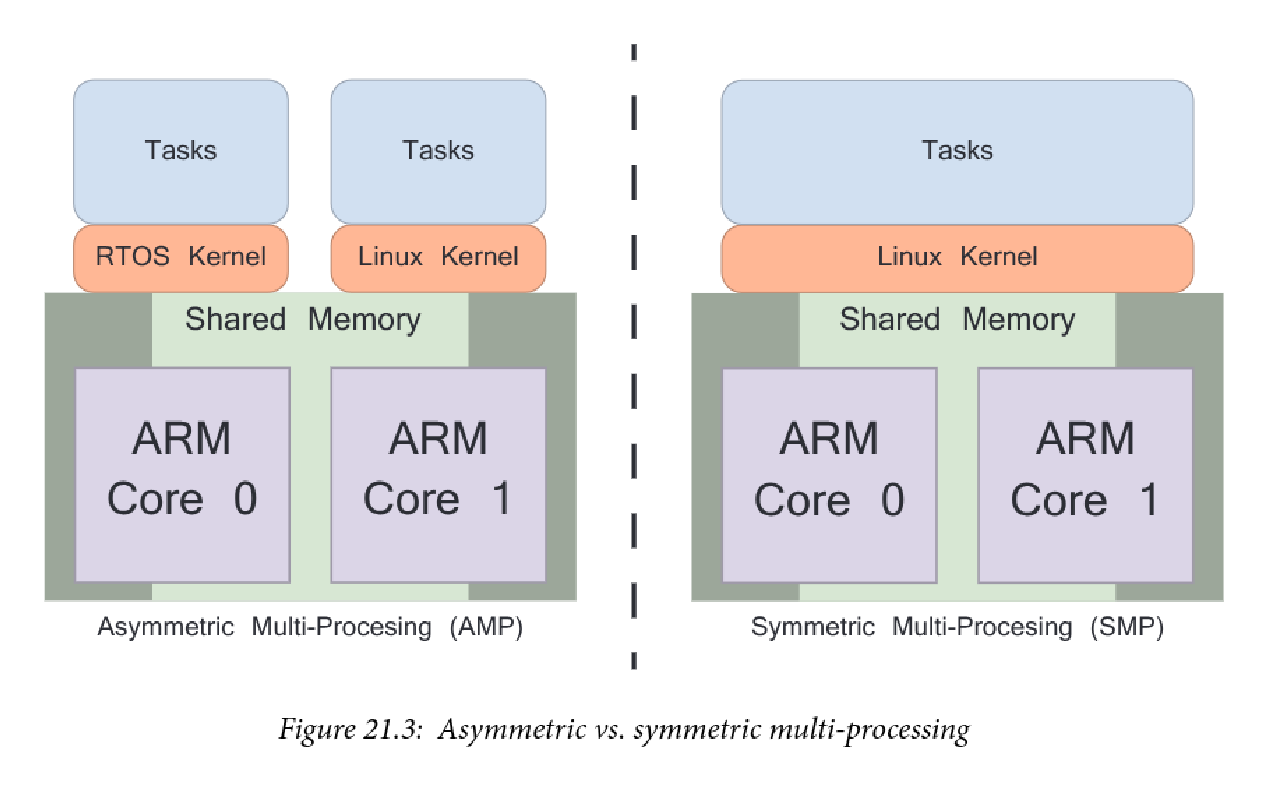
\includegraphics{cap10_amp_smp}
\caption[Procesamiento AMP y SMP]{%
Comparación de procesado AMP vs.\ SMP para el mismo procesador ARM de 2 \emph{cores}.
Extraído de~\cite{Crockett2014}.\label{f:sw-amp-smp}}
\end{figure}

La primera es cómo vamos a utilizar los diferentes \emph{cores} presentes, y tenemos
varias opciones: en la Fig.~\ref{f:sw-espectro-smp-amp} se presentan ejemplos
de sistemas operativos y su posición en el espectro.

\begin{figure}[H]
\centering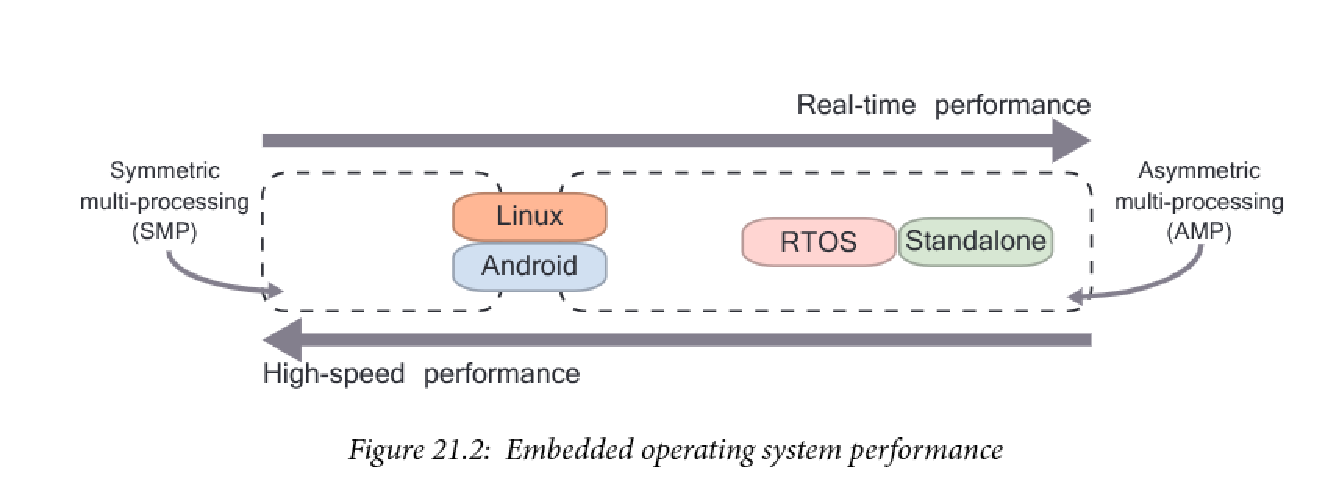
\includegraphics{cap10_espectro_smp_amp}
\caption[Ejemplos de OS en el espectro SMP-AMP]{%
Ejemplos de OS y posición en el espectro SMP-AMP. Standalone representa el
punto más extremo en \emph{real-time}; RTOS es un SO orientado a aplicaciones
\emph{real-time}.\label{f:sw-espectro-smp-amp}}
\end{figure}

\subsection{Elección del sistema operativo}
\label{S:sw-eleccion-os}

La más importante es nuestro requerimiento en tiempo de respuesta del OS, en
particular la \textbf{latencia de acceso en el peor caso}. Esto es esencial para
aplicaciones que requieren tiempos de respuesta mínimos, como accionadores
mecánicos. Las opciones principales de sistemas operativos se presentan en la
Tabla~\ref{t:sw-alternativas-os}.

\begin{table}[H]
\centering
\caption[Comparación de OS posibles en latencia]{%
Tabla comparativa de OS posibles en latencia.\label{t:sw-alternativas-os}}
\small
\begin{tabularx}{\textwidth}{|>{\raggedright\arraybackslash}p{0.17\textwidth}%
  |>{\raggedright\arraybackslash}p{0.15\textwidth}%
  |>{\raggedright\arraybackslash}X|>{\raggedright\arraybackslash}X%
  |>{\raggedright\arraybackslash}p{0.14\textwidth}|}
\hline \encabezado \textbf{Opción} & \textbf{Configura\-ción típica en Zynq} &
  \textbf{Latencia de peor caso} & \textbf{Qué provee} &
  \textbf{Costo de desarrollo} \\ \hline
\textbf{Standalone} (\emph{bare-metal}) & un núcleo, o AMP & determinística: no
  hay nada entre el programa y el hardware & \emph{drivers} básicos de Xilinx (BSP); no
  hay red, archivos ni procesos & alto: todo se escribe a mano, en C \\ \hline
\textbf{FreeRTOS} & AMP & acotada y garantizada por diseño & \emph{scheduler}
  por prioridades, colas, semáforos; red y sistema de archivos como bibliotecas
  aparte & medio-alto \\ \hline
\textbf{Linux de propósito general} & SMP & sin cota & procesos, memoria
  virtual, red, sistema de archivos, Python, ssh & bajo \\ \hline
\end{tabularx}
\end{table}

Todos los requerimientos sensibles en latencia se transfirieron al PL, así que
la opción de \emph{high-speed performance} es más que ideal como punto de
partida. En nuestro caso utilizamos el sistema operativo desarrollado por el
equipo de Pitaya. Esto no es del todo un requerimiento obligatorio, pero nos
provee un conjunto de facilidades realmente considerables, con modificaciones al
\emph{kernel mainline} (este es el base) y con adiciones sobre la capa de
usuario.

\subsection{Facilidades del Linux}
\label{S:sw-facilidades-linux}

Los servicios más importantes del mismo se presentan en la
Fig.~\ref{f:sw-kernel-linux}; estos incluyen el manejo de la memoria virtual, la
estructura de procesos (flujo de ejecución) y el \emph{scheduler}, y los \emph{drivers}
de IO de red y de memoria primaria y secundaria.

\begin{figure}[H]
\centering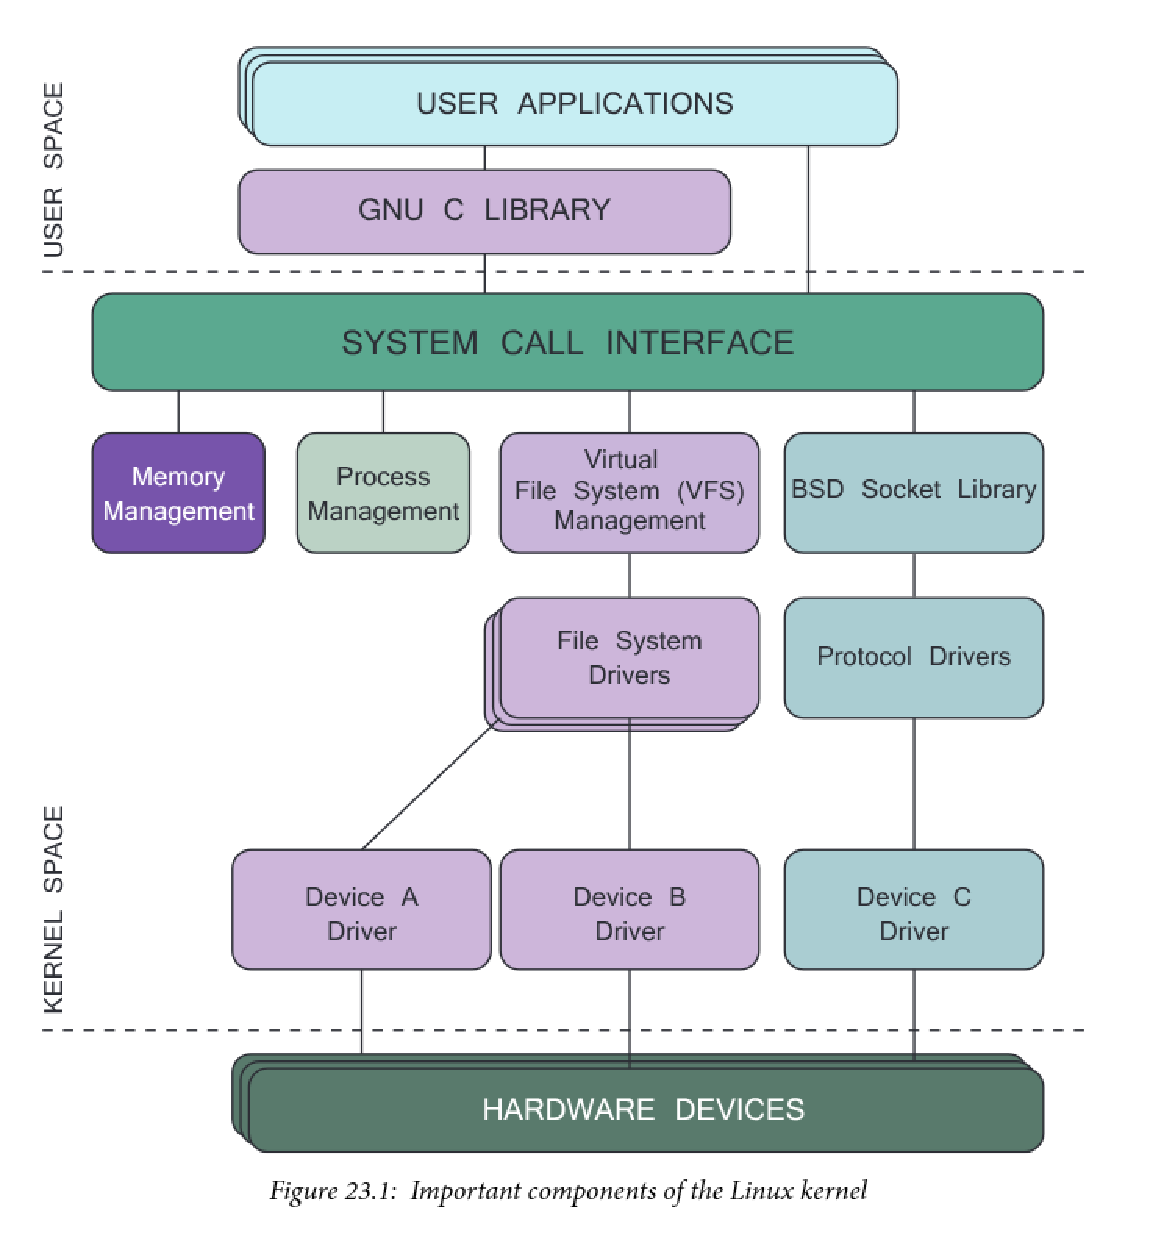
\includegraphics{cap10_kernel_linux}
\caption[Componentes del \emph{kernel} de Linux]{%
Listado de componentes del \emph{kernel} de Linux.\label{f:sw-kernel-linux}}
\end{figure}

El \textbf{\emph{kernel}} de Linux es el código del sistema operativo: esto incluye el
conjunto de estructuras internas y las APIs definidas para el manejo del mismo,
y no necesariamente incluye los \emph{drivers} particulares del HW presente. Pero al
compilar el sistema operativo (es un programa en C compilable como cualquier
otro) todos estos elementos se traducen en código máquina para el \emph{host} deseado.

\subsection{Funcionalidades de software presente}
\label{S:sw-funcionalidades}

En la Tabla~\ref{t:sw-facilidades} se presentan las funcionalidades presentes y
utilizadas en este proyecto. Estas son extremadamente útiles porque ya plantean
la base de cómo manejar el SW desde la capa de usuario, mucho más fácil para el
desarrollo acelerado. Es más, los primeros seis meses de trabajo con este
proyecto se estuvo trabajando con la modificación de un \emph{bootloader} para el
proyecto de Pavel Demin, que utiliza una distribución del tipo Alpine,
especializada para embebidos. Todo ese esfuerzo fue infructuoso, pero nos enseñó
lo importante que es tener estas funcionalidades elementales funcionando de
forma correcta para comenzar un desarrollo mínimo.

\begin{table}[H]
\centering
\caption[Facilidades del SW que provee la distribución de Pitaya]{%
Tabla de facilidades del SW que provee la distribución de Pitaya de
antemano.\label{t:sw-facilidades}}
\small
\begin{tabularx}{\textwidth}{|>{\raggedright\arraybackslash}p{0.27\textwidth}%
  |>{\raggedright\arraybackslash}X|>{\raggedright\arraybackslash}p{0.15\textwidth}|}
\hline \encabezado \textbf{Facilidad} & \textbf{Beneficio} &
  \textbf{Quién la provee} \\ \hline
\textbf{\ruta{/dev/mem} + \codigo{mmap}} & acceder al PL sin escribir un \emph{driver}
  particular & \emph{kernel} (\emph{mainline}) \\ \hline
Ubuntu ARM + Python 3.10 + NumPy & un entorno de trabajo completo en la placa,
  sin compilar nada & distribución \\ \hline
\codigo{systemd}, ssh, rsync & servicios que arrancan solos y despliegue por
  red & distribución \\ \hline
\emph{Bootloader} & FSBL generado para este PS7, U-Boot, \emph{kernel} 5.15-xilinx y el
  \emph{device tree} de \textbf{esta} placa, todo armado. Es el ítem más valioso de la
  lista y el que más trabajo ahorra & \\ \hline
API de \emph{deep memory} (\codigo{rp\_AcqAxi*}) & capturar a DDR por los
  puertos HP desde la librería, sin RTL propio & \\ \hline
Las regiones de DDR ya reservadas & \codigo{buffer@1000000} (2~MB, para la
  \emph{deep memory}) y \codigo{labuf@a000000} (32~MB, del analizador lógico),
  en el \emph{device tree} de fábrica & \\ \hline
\textbf{\codigo{fpgautil}} (\ruta{/opt/redpitaya/bin/}) & programa la PL y
  aplica el \emph{overlay} de \emph{device tree} en un comando & \\ \hline
\textbf{\codigo{monitor}} (\ruta{/opt/redpitaya/bin/}) & leer/escribir un
  registro de la PL desde la \emph{shell}, y con \codigo{-f} el \textbf{modelo de placa
  grabado en la EEPROM} & \\ \hline
\textbf{\codigo{scpi-server}} (TCP 5000) & manejar la placa como un instrumento
  de banco desde MATLAB, LabVIEW o Python & \\ \hline
\end{tabularx}
\end{table}

A continuación describimos algunos errores encontrados a nivel de HW
(especialmente en el proyecto de Pitaya) y cómo los evitamos.

\subsection{Modos de fallo en el HW implementado}
\label{S:sw-modos-fallo}

Todo el software trabaja dentro del espacio de usuario: no escribimos un \emph{driver}
propio, sino que hacemos uso del \emph{device} \ruta{/dev/mem}, que representa la
memoria física, dentro del espacio de direcciones del proceso.
\begin{enumerate}
  \item \textbf{Lecturas masivas}: no se limita el tipo de operaciones que puede
    hacer el PS sobre la región de memoria del PL; en especial, el modelo de
    memoria \emph{Device} únicamente habla del reordenamiento y de las propiedades de
    cacheo. No se impide que el compilador emita instrucciones de acceso
    múltiple (\codigo{LDM}/\codigo{STM}) o de NEON. Muchos de los \emph{drivers} de
    Linux traducen estas instrucciones en transferencias de alto \emph{throughput}, con
    ráfagas o accesos anchos, las cuales nuestro \emph{slave} en el PL no acepta. Este
    rechazo es un tipo de bus \emph{fault} presentado internamente con un código de
    \emph{external abort}, escalando hasta un error fatal que \textbf{reinicia
    el sistema}.
\end{enumerate}

La existencia de estos modos de fallo según la utilización del usuario es lo que
impulsa la creación de un \emph{driver} en el espacio del \emph{kernel}. Esto no es más que
seguir la API del sistema operativo en cuestión; nosotros vamos a implementar
una API propia en el espacio de usuario que evita los modos de falla
identificados.

%==============================================================================
\section{API: \emph{Application Programming Interface}}
\label{S:sw-api}

Esta es la librería con la que podemos acceder a diversos tipos de
\textbf{registros, algoritmos y funcionalidades} en SW en el espacio de usuario
(no del \emph{kernel}). Para esta utilizamos una estructura extremadamente similar a la
que emplea el proyecto original de Pitaya. En la Fig.~\ref{f:sw-capas} se
presentan los 6 niveles de la \textbf{jerarquía de dependencias} de este
software, en el sentido de que las capas superiores utilizan las capas
inferiores. La misma consta de un \emph{driver} escrito en C++ en la capa de usuario
(capas 1--4, en color rojo), mientras que los bloques azules son
\emph{bindings} a Python.
\begin{enumerate}
  \item \textbf{Mapeo crudo}: se utiliza el dispositivo \ruta{/dev/mem} y
    \codigo{mmap} para acceder a regiones físicas.
  \item \textbf{Acceso a palabras}:
  \begin{itemize}
    \item Se definen transacciones de 32 bits (el ancho de bus presente) con las
      funciones \codigo{w32} / \codigo{r32} / \codigo{\_read\_words}, en Python
      mediante la librería \codigo{ctypes}, para las regiones de memoria
      asociadas al bus de Pitaya. Gracias a esto no tenemos el modo de falla por
      ancho de palabras explicado en la Sec.~\ref{S:sw-modos-fallo}.
    \item Para otras direcciones se pueden implementar accesos más anchos. En
      este proyecto no se lo implementó.
  \end{itemize}
  \item \textbf{\emph{Handlers}}: son clases \textbf{compartidas por todo el sistema},
    generalmente del tipo \emph{singleton}. Debido a que son compartidas por todo el
    sistema, generalmente se las asocia al sistema operativo (esto sería un
    \emph{driver} en la capa de OS). Sin embargo, podemos manipularlas en el espacio de
    usuario con cualquier lenguaje de programación que deseemos: podríamos hacer
    una clase en Python equivalente para manipular el \emph{handler} descrito en
    nuestra librería en C o, mejor aún, utilizar el código fuente de la
    librería para compilar un código análogo pero en Python. Esto es lo que hace
    el \emph{binding}.
  \item \textbf{Métodos de \emph{handlers}}: adquisición y configuración.
  \begin{itemize}
    \item Implementan los bucles de adquisición presentados en los Caps.~\ref{C:implmca} y~\ref{C:osc}.
    \item El sistema devuelve el dato con un formato \textbf{conocido} en tiempo
      de ejecución.
  \end{itemize}
  \item \textbf{Código de sesión y fuentes}: guardado continuo de eventos y
    resumen.
  \begin{itemize}
    \item Abstracciones que utilizamos para agregar las fuentes y receptores de
      información presentes.
  \end{itemize}
  \item \textbf{Aplicaciones}: \emph{scripts} que utilizan cualquiera de las
    funcionalidades previas.
\end{enumerate}

\begin{figure}[H]
\centering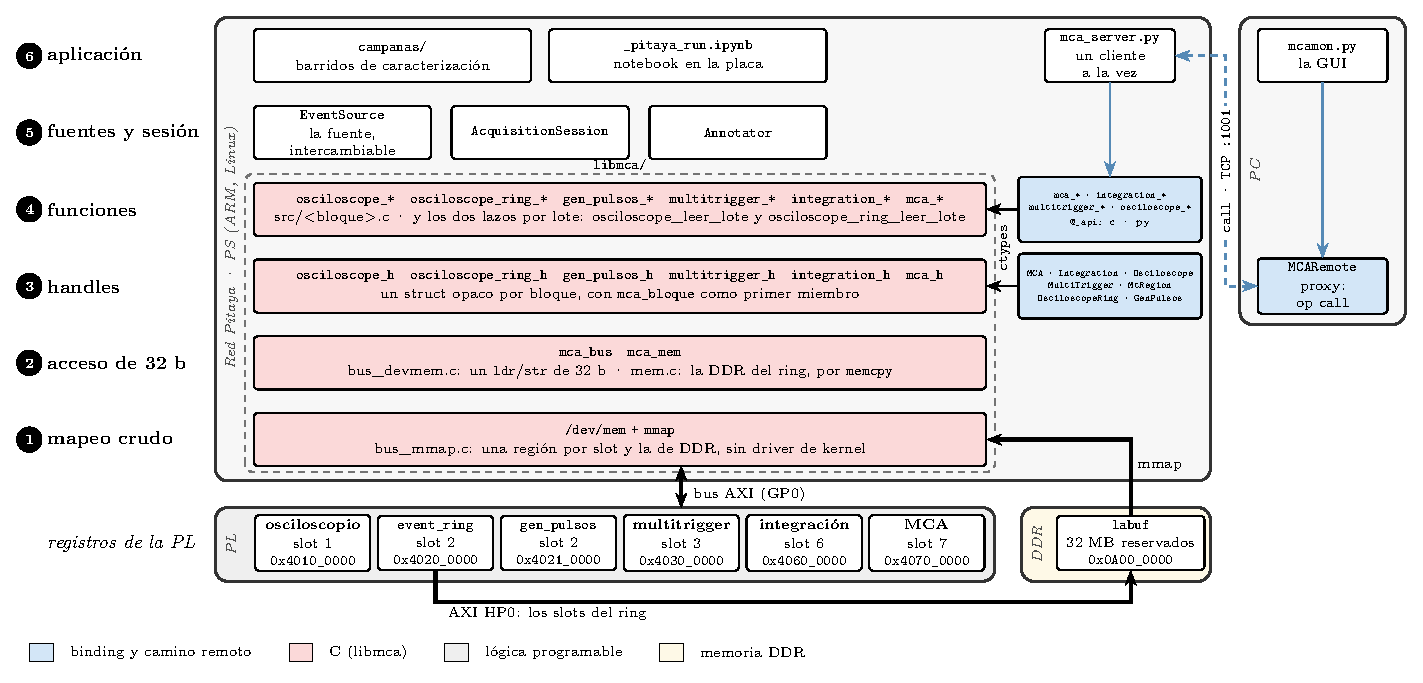
\includegraphics{cap10_niveles}
\caption[Capas de abstracción del SW]{%
Capas de abstracción de SW desarrolladas para este proyecto.\label{f:sw-capas}}
\end{figure}

Los \emph{handles} son clases del tipo \emph{singleton} porque, si no, podemos tener dos
procesos que operan sobre la misma región de memoria compartida (el rango de
direcciones de un módulo) sin un esquema de contención previamente acordado. Un
primer acercamiento podría ser configurar que la región pueda ser mapeada una
única vez. Esto no resulta beneficioso porque sería una denegación total a un
proceso, de forma que resultaría en un error en tiempo de compilación, lo cual
no es deseado. La otra es darle la capacidad de acceder a ese recurso, pero
mediante un objeto compartido y único que se encargue de implementar la
contención y el reparto del servicio: este patrón es el \emph{singleton}.

La ventaja de dividirlo por secciones en estos seis niveles es que podemos
realizar \emph{tests} para cada una de las capas individuales (\emph{unit testing}).
Para el funcionamiento correcto de la API se necesita cargado el \emph{bitstream} del
HW correcto, el que diseñamos; esto incluye la versión de los módulos
individuales y la del \emph{top} de integración. En la Sec.~\ref{S:ap-sw-bitstream}
se presentan más detalles.

%==============================================================================
\section{\emph{Driver} en C++: \texorpdfstring{\texttt{libmca}}{libmca}}
\label{S:sw-libmca}

Se llama \codigo{libmca}, pero cuenta con \emph{handlers} para todos los submódulos
instanciados dentro del módulo de integración. La idea principal consiste en
asociar cada recurso compartido a una estructura \emph{singleton} dada; por esto
planteamos:
\begin{itemize}
  \item Nivel 1, el mapeo: se abre \ruta{/dev/mem} y se mapea la región física
    de un \emph{slot} con \codigo{mmap}. El único archivo que accede a los registros
    del PL es \ruta{bus_devmem.c}, y se comprueba al compilar que no emita
    instrucciones de acceso múltiple.
  \item Nivel 2, el acceso por palabras:
  \begin{itemize}
    \item \codigo{mca\_bus}: implementa el acceso al bus \emph{custom}, asegurando el
      tipo de acceso. Tiene dos \emph{backends}: \codigo{devmem}, el real, y uno por
      \emph{callbacks}, que usan los \emph{tests} y el modelo sin placa. Operaciones
      principales:
    \begin{itemize}
      \item \codigo{mca\_bus\_open\_devmem()} mapea la subregión del \emph{slot}, y
        \codigo{mca\_bus\_close()} libera el mapeo.
      \item El acceso por palabra: \codigo{w32()}/\codigo{r32()}, y
        \codigo{read\_words()}, que lee $n$ palabras de a una, nunca como
        ráfaga.
      \item Verifica la alineación y el rango de cada acceso antes de llegar al
        \emph{backend}.
    \end{itemize}
    \item \codigo{mca\_mem}: el acceso a la región de DDR que escribe el ring.
      Es un tipo aparte porque no tiene la restricción del bus: se copia de a
      bloques, y por eso es rápido. Se mapea sin caché, porque los puertos HP no
      son coherentes con la caché.
  \end{itemize}
  \item Nivel 3, los \emph{handles}: \codigo{mca\_bloque} es la base común de todos
    ellos (el bus, si el \emph{handle} es dueño de él, y el último error), y cada
    \codigo{*\_regs.h} contiene el mapa de registros de su bloque. Al abrir un
    \emph{handle} se comprueba el \emph{magic} del bloque.
\end{itemize}

Los detalles de estas clases se presentan en la Fig.~\ref{f:sw-clases-base};
esta figura también muestra la existencia de \codigo{mca\_api.h}, que contiene
la \emph{metadata} de la versión de la API y los códigos de error de las llamadas a las
funciones. En la parte superior aparece cómo utilizar esta librería: a la
derecha, la forma estándar de C mediante un \codigo{\#include}, y a la
izquierda, la forma según el \emph{binding} de Python, que la incluye mediante un
\codigo{import}.

\begin{figure}[H]
\centering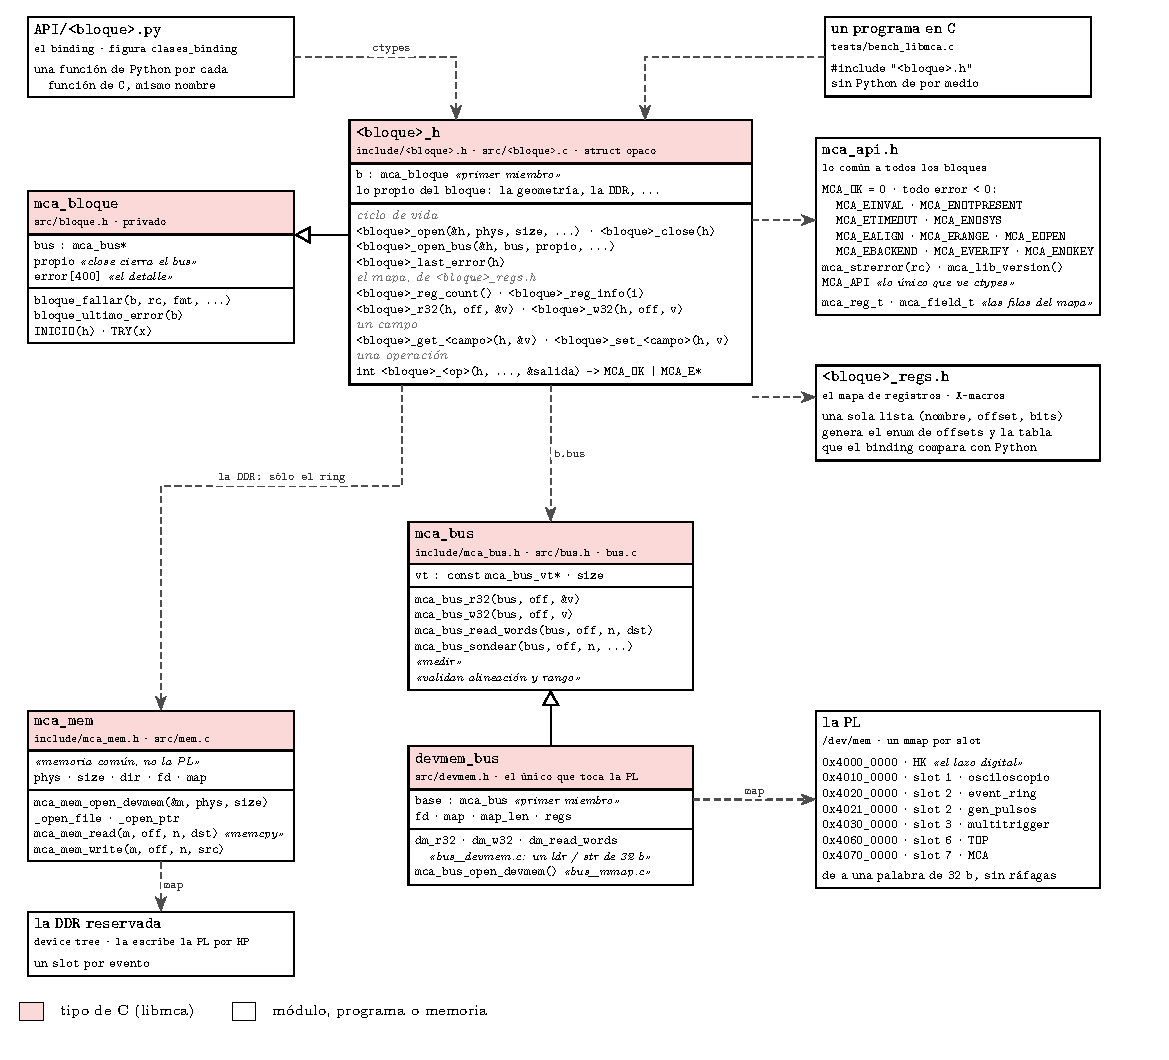
\includegraphics{cap10_clases_bloque}
\caption[Clases base de \codigo{libmca}]{%
Clases base de \codigo{libmca}. El \emph{handle} con \codigo{mca\_bus} representa el
bloque fundamental para representar los \emph{slots} de la integración\label{f:sw-clases-base}}
\end{figure}

\subsection{Bloques implementados y métodos de \emph{handlers}}
\label{S:sw-bloques}

En la Fig.~\ref{f:sw-bloques} se presentan todos los bloques definidos para este
proyecto: todos son clases derivadas de \codigo{mca\_bloque}, y se presentan los
métodos especializados para cada uno. La API implementada en este proyecto sigue
la nomenclatura \codigo{\textless módulo\textgreater\_\textless capa\textgreater\_\textless campo\textgreater} para las funciones. En la
Tabla~\ref{t:sw-api-nombres} se presentan ejemplos en cada uno de estos niveles.

\begin{figure}[H]
\centering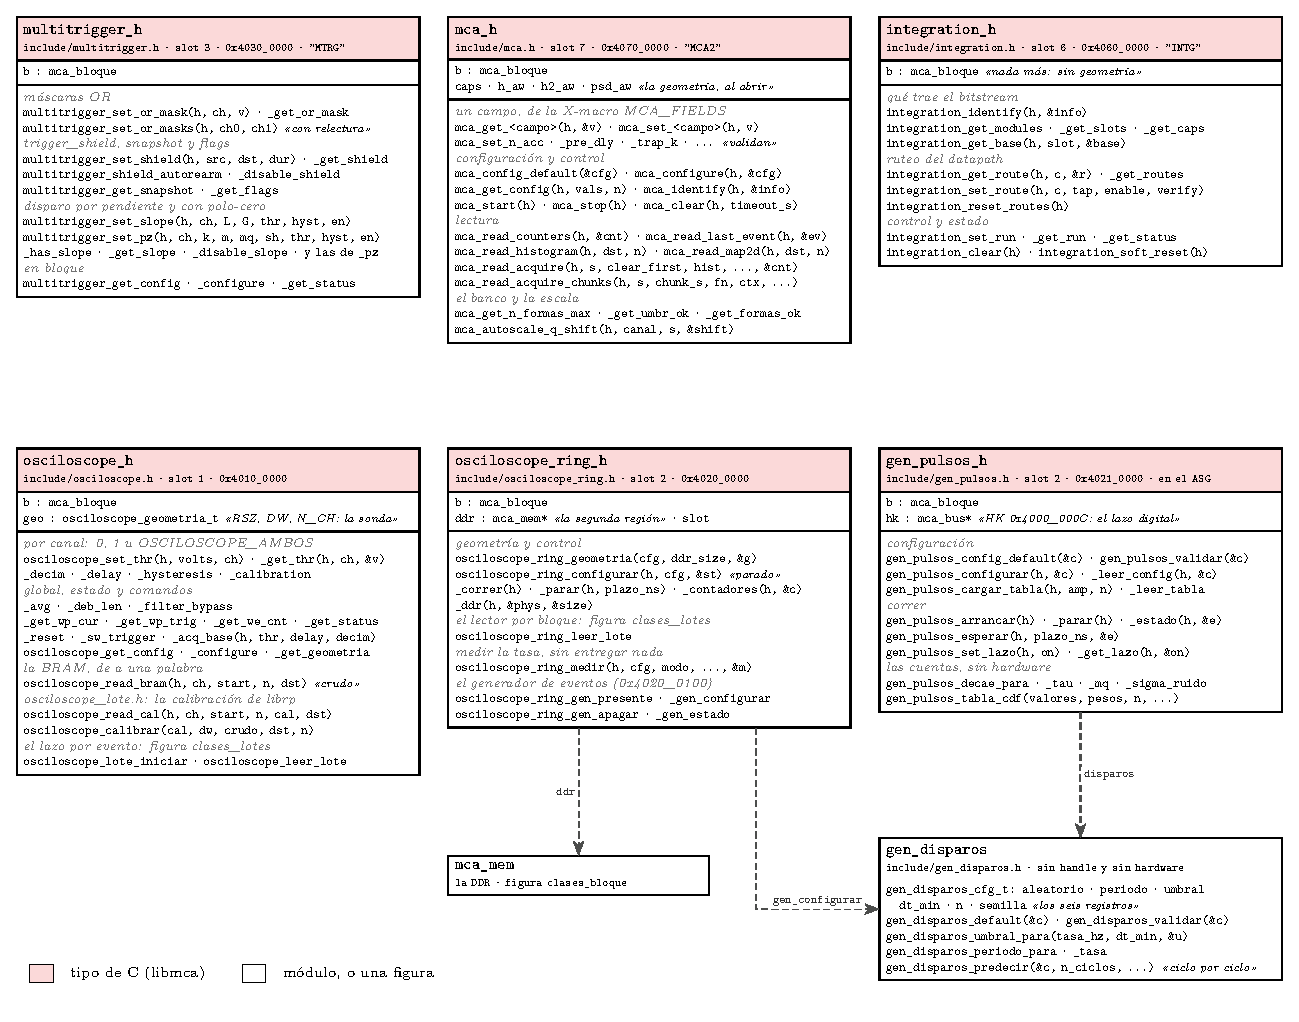
\includegraphics{cap10_clases_libmca}
\caption[Clases fundamentales de \codigo{libmca}]{%
Clases fundamentales en la librería \codigo{libmca}. Se presentan las clases
\codigo{multitrigger}, \codigo{mca}, \codigo{integracion},
\codigo{osciloscope}, \codigo{osciloscope\_ring} y
\codigo{gen\_pulsos}.\label{f:sw-bloques}}
\end{figure}

\begin{table}[H]
\centering
\caption[Estructura de nombres de la API]{%
Estructura de nombres de la API.\label{t:sw-api-nombres}}
\small
\begin{tabularx}{\textwidth}{|l|>{\raggedright\arraybackslash}p{0.3\textwidth}%
  |>{\raggedright\arraybackslash}X|}
\hline \encabezado \textbf{Capa} & \textbf{Qué dice} & \textbf{Valores}
  \\ \hline
1 $\cdot$ módulo & bloque que utiliza & \codigo{mca\_} $\cdot$
  \codigo{osciloscope\_} $\cdot$ \codigo{osciloscope\_ring\_} $\cdot$
  \codigo{multitrigger\_} \\ \hline
2 $\cdot$ tipo de API & clase de operación & cfg/\emph{status} $\cdot$
  \codigo{read\_} $\cdot$ \codigo{write\_file\_} / \codigo{save\_file\_}
  \\ \hline
3 $\cdot$ campo & el registro o la operación concreta & \codigo{thr},
  \codigo{gate\_long}, \codigo{histogram}, \ldots \\ \hline
\end{tabularx}
\end{table}

Muchos de estos elementos tienen estructuras internas, por ejemplo
\codigo{osciloscope\_lote\_t}, que no se detallan en profundidad en este
trabajo, pero se nombran en la Tabla~\ref{t:ap-sw-estructuras} de la
Sec.~\ref{S:ap-sw-estructuras}.

\subsection{Adquisición de un evento mediante la API}
\label{S:sw-adquisicion}

Tenemos un ciclo de software que \textbf{abstrae} la implementación específica
del flujo de adquisición. En el módulo osciloscopio, por ejemplo, el flujo es el
mismo con las dos interfaces de comunicación, la BRAM y el ring en DDR, aunque
cada una tiene su propio mecanismo de transferencia. La API se encarga de los
pasos que dependen de la implementación; estos se describen en la
Sec.~\ref{S:osc-flujo-basico} (BRAM), la Sec.~\ref{S:osc-uso-anillo} (ring) y
la
Sec.~\refpend{S:implmca-flujo}{Implementación del MCA: flujo de utilización del
módulo} para cada módulo.

Hay que ver qué pasa con una traza del osciloscopio después de leerla. En la
Fig.~\ref{f:sw-lazos}(a) y (b), C la escribe directamente en la fila siguiente
de un \textbf{\emph{batch}}, una estructura que se reserva una sola vez al arrancar la
corrida. No es un \emph{append}: no se copia ni se reserva memoria por evento, y
Python interviene una sola vez por \emph{batch}. Los \emph{batches} son siempre los mismos
objetos y circulan entre dos hilos: el lector, que los llena, y el escritor, que
los guarda.

\begin{figure}[H]
\centering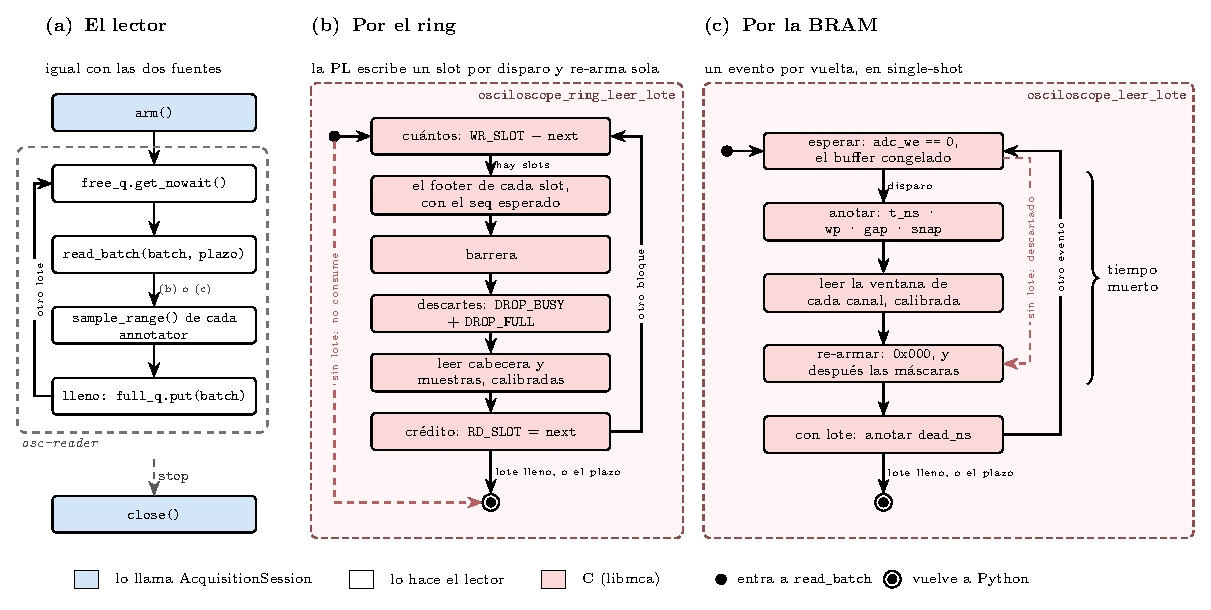
\includegraphics{cap10_maquinas_estados}
\caption[Lazos de adquisición por software]{%
Lazos de adquisición por software. (a) El osciloscopio por la BRAM: Python llama
a \codigo{arm()} una vez, a \codigo{read\_batch()} una vez por \emph{batch} y a
\codigo{close()} al final. Adentro de \codigo{read\_batch}, \codigo{libmca} lee
un evento por vuelta, en C y sin el GIL, y re-arma el osciloscopio después de
cada uno. (b) El osciloscopio por el ring: el mismo lazo de Python; adentro, un
bloque de \emph{slots} por vuelta, y nadie re-arma desde el PS.\label{f:sw-lazos}}
\end{figure}

\subsection{\emph{Binding} y clases de sesión Python}
\label{S:sw-binding}

Esta es una capa que expone cada función de C como una función de Python, con el
mismo nombre y los mismos argumentos; funciona a partir de linkear el binario
compilado \ruta{libmca.so}. Sólo traduce los tipos (enteros, structs, arreglos
de NumPy) y convierte los códigos de error de C (\codigo{MCA\_E*}) en las
excepciones habituales de Python (\codigo{ValueError}, \codigo{TimeoutError},
\codigo{KeyError}). Sobre esta se construye el software de captura de eventos
del osciloscopio. Sus clases separan qué se captura, \textbf{qué se agrega a cada
evento} y \textbf{cómo se coordina la corrida}:
\begin{enumerate}
  \item \textbf{\codigo{EventSource}, la fuente.} Define cuándo ocurre un evento
    y entrega su traza. No es una clase base sino una interfaz: sirve como
    fuente cualquier objeto con los métodos \codigo{arm()},
    \codigo{read\_batch()}, \codigo{close()} y \codigo{meta()}. Hay dos
    implementaciones:
  \begin{itemize}
    \item \codigo{BramSource} lee la ventana de cada evento de la BRAM del
      osciloscopio;
    \item \codigo{RingSource} lee los eventos que el event\_ring dejó en la DDR.
  \end{itemize}
    En las dos, el lazo que espera el disparo y lee los datos está en C, y cada
    llamada entrega un lote entero de eventos.
  \item \textbf{\codigo{Annotator}, los anotadores.} Agregan a cada evento
    columnas que no vienen de la fuente:
  \begin{itemize}
    \item Valores constantes de la corrida (\codigo{ConstantAnnotator});
    \item Mediciones lentas, como una temperatura o una posición, que un hilo
      propio lee y deja en una caché (\codigo{CachedAnnotator}).
  \end{itemize}
  \item \textbf{\codigo{AcquisitionSession}, la sesión.} Coordina una corrida
    completa:
  \begin{itemize}
    \item Arma el esquema del evento a partir de la fuente y los anotadores;
    \item Reserva un \emph{pool} de lotes (\codigo{EventBatch}) según un presupuesto de
      RAM, preasignados por el OS;
    \item Lanza dos hilos: el lector (\codigo{ReaderThread}), que llena lotes
      desde la fuente, y el escritor (\codigo{ChunkWriter}), que guarda en disco
      cada lote lleno.
  \end{itemize}
\end{enumerate}
En la Fig.~\ref{f:sw-clases-sesion} se presenta el diagrama de clases.

\begin{figure}[H]
\centering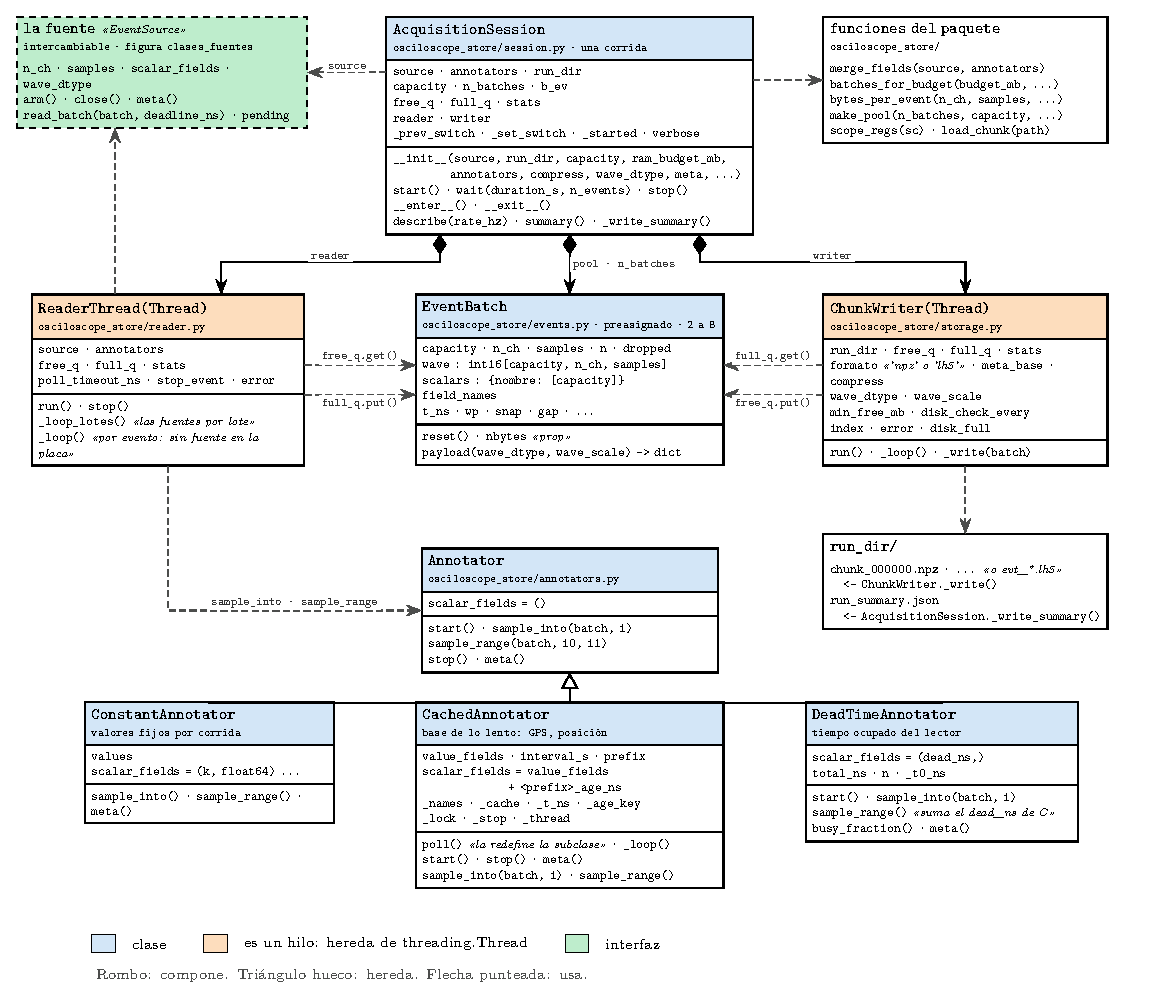
\includegraphics{cap10_clases_sesion}
\caption[Clases de sesión en Python]{%
Clases de sesión, implementadas en Python.\label{f:sw-clases-sesion}}
\end{figure}

La utilización de este \emph{binding} tiene un costo fijo por llamada, que medimos en
la Sec.~\ref{S:sw-bench-libmca}. Como el costo es por llamada y no por dato,
deja de importar cuando una llamada hace mucho trabajo. Por esto mismo decidimos
crear las clases de sesión y de manejo de archivos y eventos en Python: la
complejidad de tener todo en C no valía la pena.

%==============================================================================
\section{Guardado de archivos para el MCA y el OSC}
\label{S:sw-guardado}

Una adquisición deja dos tipos de archivos: los espectros del MCA y los eventos
del osciloscopio. En esta sección describimos qué guarda cada uno, cómo es el
archivo, cómo y dónde se escribe, y qué parte del software lo hace.

A continuación describimos los \textbf{formatos de guardado} de cada módulo.
\begin{itemize}
  \item Módulo \textbf{MCA}:
  \begin{itemize}
    \item Generalmente no necesitamos analizar la evolución del histograma con
      el tiempo: queremos su forma final. La API acumula siempre en el mismo
      histograma, y \codigo{mca\_read\_acquire\_chunks} llama a una función del
      programa cada \codigo{chunk\_s} segundos. Con eso, un programa puede
      sobrescribir el mismo archivo durante la medición o guardar los
      histogramas parciales y analizar su variación.
    \item Dada la poca cantidad de datos, el formato por defecto es
      \emph{human-readable}: un \textbf{csv} con una cabecera
      \codigo{\# clave: valor} que lleva la versión del esquema y los parámetros
      de adquisición.
    \item Implementamos además el estándar \textbf{ANSI N42.42-2011}, que abren
      otros programas de espectroscopía. Sólo admite el espectro 1D: el mapa 2D
      no entra en el formato.
    \item Hay también un \ruta{.npz} y un \ruta{.json}. \codigo{mca\_load\_file}
      lee los cuatro formatos y devuelve siempre el histograma y su \emph{metadata},
      así que el formato no cambia el análisis.
  \end{itemize}
  \item Módulo \textbf{OSC}:
  \begin{itemize}
    \item Guardamos un archivo por \emph{batch}: 4096 eventos por defecto, unos
      0.6~MB con dos canales de 32 muestras. Cada archivo se escribe con un
      nombre temporal y se renombra al terminar (\ruta{.tmp} +
      \codigo{os.replace}), así que todo archivo visible está completo. Al
      cerrar la corrida se escribe además un resumen,
      \ruta{run\_summary.json}, con los totales.
    \item Implementamos dos formatos. Uno es \textbf{LH5}, el formato basado en
      HDF5 (\emph{Hierarchical Data Format}) que usa la colaboración LEGEND
      para los datos de sus detectores de germanio~\cite{LEGENDHDF5}: lo abre
      su lector oficial sin saber nada de este proyecto, pero escribe más lento.
      El otro, el formato por defecto, es el \ruta{.npz} de
      NumPy~\cite{NumpyNEP1}: sólo necesita NumPy y es el más rápido.
  \end{itemize}
\end{itemize}

Como los sistemas de adquisición trabajan de forma independiente en HW, estos
pueden ser leídos en forma independiente. Por esto tenemos un mca-writer y un
\codigo{AcquisitionSession}. En la Tabla~\ref{t:sw-archivos} se presentan los
diferentes archivos de salida.

\begin{table}[H]
\centering
\caption[Estructura de los archivos guardados]{%
Estructura de archivos guardados.\label{t:sw-archivos}}
\small
\begin{tabularx}{\textwidth}{|>{\raggedright\arraybackslash}p{0.2\textwidth}%
  |>{\raggedright\arraybackslash}X|>{\raggedright\arraybackslash}p{0.32\textwidth}|}
\hline \encabezado \textbf{Formato} & \textbf{Estructura} & \textbf{Escritor}
  \\ \hline
\codigo{chunk\_\%06d.npz} & \codigo{wave} int16 \codigo{(eventos, canal,
  muestra)} + una columna por campo escalar + \codigo{meta} como \emph{array} 0-d &
  \codigo{ChunkWriter} \\ \hline
\codigo{evt\_\%06d.lh5} & lo mismo en LH5: una tabla \codigo{raw} con las columnas
  y una \codigo{waveform\_inN} por canal, y \codigo{meta} como texto JSON &
  \codigo{ChunkWriter} \\ \hline
\ruta{run_summary.json} & los totales de la corrida &
  \codigo{AcquisitionSession} \\ \hline
\ruta{.csv} & el espectro con la \emph{metadata} en cabecera \codigo{\#}; \textbf{el
  formato por defecto}, se abre en Excel u Origin &
  \codigo{mca\_write\_file\_histogram} \\ \hline
\ruta{.npz} / \ruta{.json} & el espectro estructurado &
  \codigo{mca\_save\_file\_*} \\ \hline
\end{tabularx}
\end{table}

Para aprovechar el formato binario del \ruta{.npz} vamos a necesitar un programa
de lectura; este está incluido en la API, con la estructura de datos deseada.

\subsection{Contenido de los archivos de trazas del osciloscopio}
\label{S:sw-contenido-trazas}

Una corrida del osciloscopio es una tabla de eventos, con la misma configuración
de principio a fin. Cada evento tiene:
\begin{itemize}
  \item \textbf{La ventana del evento}: las muestras alrededor del disparo;
  \item \textbf{Sus datos escalares}, que cambian en cada evento y declara la
    fuente: cuándo llegó (\codigo{t\_ns}), dónde estaba el puntero de escritura
    (\codigo{wp}), qué fuente disparó (\codigo{snap}) y cuántos eventos se
    descartaron antes (\codigo{gap});
  \item \textbf{Las columnas de los anotadores}: el tiempo muerto
    (\codigo{dead\_ns}), valores fijos de la corrida, o mediciones lentas, como
    una temperatura, con su antigüedad (\codigo{\textless p\textgreater\_age\_ns}).
\end{itemize}
La tabla se parte en archivos de un \emph{batch} cada uno (4096 eventos por defecto). Al
final se agrega un resumen de la corrida, \ruta{run_summary.json}.

\subsubsection{Trazas en formato \texorpdfstring{\texttt{.npz}}{.npz}}

Cada \emph{batch} lleno se guarda en un archivo \ruta{chunk_NNNNNN.npz}, numerado desde
cero. Un \ruta{.npz} es un \emph{zip} con un arreglo de NumPy (\ruta{.npy}) por
entrada, cada uno con su nombre, su forma y su tipo~\cite{NumpyNEP1}.
\codigo{np.load} lo abre como un diccionario y lee cada arreglo recién cuando se
lo pide.

Estructuramos cada \emph{batch} con tres índices, \codigo{(evento, canal, muestra)},
más una columna 1D por cada metadato. El primer eje, \codigo{capacity}, es la
cantidad de eventos que entran en un \emph{batch}; \codigo{n\_ch} es la cantidad de
canales que se adquieren en paralelo, y \codigo{samples}, la muestra dentro de
la ventana. Las muestras se guardan como \codigo{int16}: son cuentas de un ADC
de 14 bits, y en \codigo{float32} ocuparían el doble. Las columnas no son fijas:
la fuente y cada annotator declaran las suyas, y el \emph{batch} se arma al arrancar la
corrida. Este esquema se presenta en la Fig.~\ref{f:sw-esquema-evento}. El
\codigo{gap} es un \codigo{uint8} y satura en 255; por eso la cuenta exacta de
descartes va en la \emph{metadata} de cada archivo. Los descartes del final de la
corrida no tienen un evento siguiente donde anotarse, así que van en
\ruta{run_summary.json}.

\begin{figure}[H]
\centering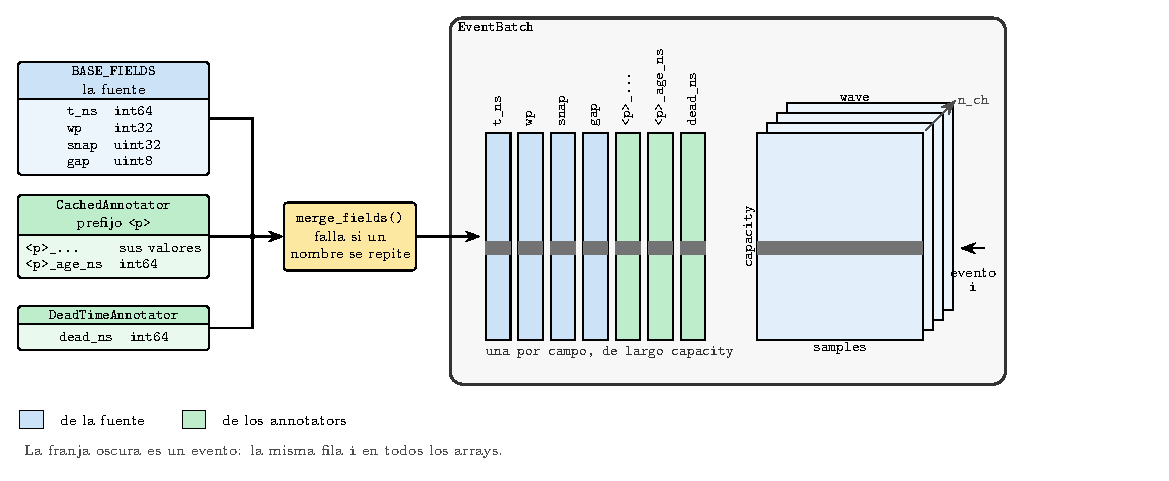
\includegraphics{cap10_esquema_evento}
\caption[Estructura de un \emph{batch} de eventos]{%
Estructura de un \emph{batch} de eventos. Es la base del guardado
automático.\label{f:sw-esquema-evento}}
\end{figure}

El formato no está hardcodeado: se puede construir en \emph{runtime} y se pueden
obtener sus campos inspeccionando \codigo{meta['schema\_version']} y
\codigo{meta['fields']}.

\subsubsection{Metodología de escritura}

El escritor guarda cada \emph{batch} apenas se llena, sin esperar a juntar varios. Para
que nunca quede a la vista un archivo a medias, primero escribe un temporal
(\ruta{chunk_000123.npz.tmp}) en la misma carpeta, y al terminar le da el nombre
final con \codigo{os.replace} (Fig.~\ref{f:sw-escritura}). Ese renombre es
atómico~\cite{Kerrisk2010} porque los dos nombres están en el mismo sistema de
archivos: otro programa ve el archivo completo o no lo ve. Por eso se puede
copiar o analizar una corrida mientras anda, y \codigo{archivos\_de\_corrida}
nunca devuelve un \ruta{.tmp}. Mientras tanto, \codigo{write()} vuelve cuando los
datos están en el page \emph{cache} del \emph{kernel}, es decir en RAM; el \emph{kernel} los pasa a la
tarjeta después. El escritor no fuerza ese paso con \codigo{fsync}. La garantía
es entonces que ningún archivo visible está incompleto, no que sobreviva a un
corte de luz~\cite{Pillai2014}. Cada 8 archivos, el escritor revisa el lugar
libre. Si quedan menos de 200~MB, para, y la sesión corta la corrida con el
motivo \codigo{disk}.

La Fig.~\ref{f:sw-escritura} muestra la secuencia: cada \emph{batch} pasa por un
\ruta{.tmp} antes de tener su nombre final, y al cerrar la corrida
\ruta{run_summary.json} sigue el mismo camino.

\begin{figure}[H]
\centering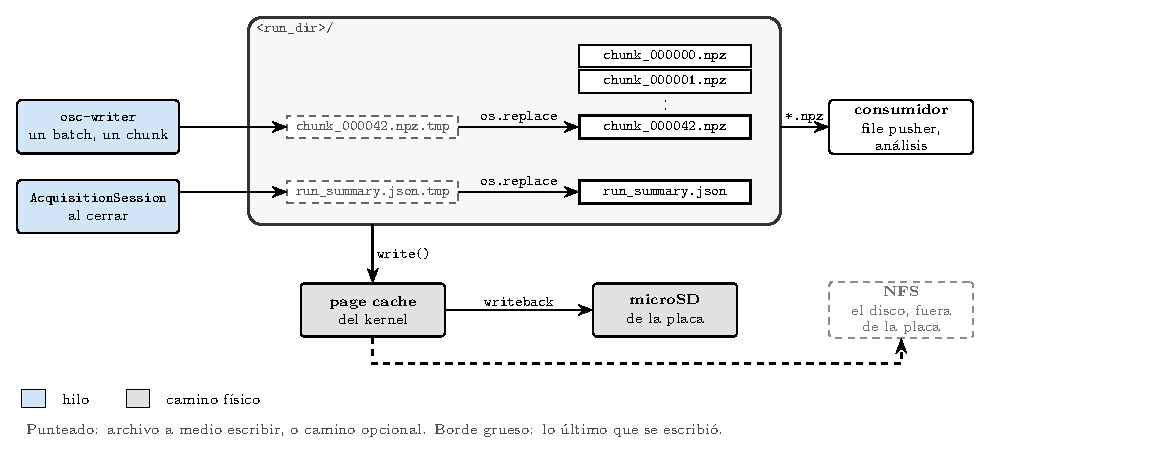
\includegraphics{cap10_escritura_corrida}
\caption[Guardado por \emph{chunks} \texttt{.npz} y resumen \texttt{.json}]{%
Metodología de guardado por \emph{chunks} \ruta{.npz} y resumen
\ruta{.json}.\label{f:sw-escritura}}
\end{figure}

\subsubsection{Localización de guardado}
\label{S:sw-localizacion}

La microSD de la placa tiene 32~GB, pero la partición del sistema tiene 6.6~GB y
quedan unos 1.4~GB libres. Más que el tamaño, limita la velocidad. La escritura
sostenida tiene un techo que no depende de la tarjeta: el controlador SD del
Zynq trabaja en modo de 4 bits con un reloj de \qty{50}{\mega\hertz}, así que el
bus llega a unos 25~MB/s. Lo que llega a la tarjeta en esta placa se presenta en
la Sec.~\ref{S:sw-bench-disco}. Para el MCA alcanza de sobra, porque un espectro
de 8192 canales ocupa 32~kB. Para el osciloscopio depende de la ventana:
\begin{itemize}
  \item \textbf{2 canales $\times$ 32 muestras} (la ventana por defecto): un
    evento ocupa 146~B. A 50~kev/s son 7.3~MB/s, por debajo de ese techo.
  \item \textbf{2 canales $\times$ 1024 muestras}: un evento ocupa 4~KiB. A
    50~kev/s son 205~MB/s, ocho veces el techo del bus. Los 1.4~GB libres se
    llenarían en \qty{7}{\second}.
\end{itemize}
La alternativa es \textbf{escribir por la red}, en un sistema de archivos NFS
montado en la placa. Para la sesión no cambia nada: \codigo{run\_dir} es
simplemente otra carpeta. Es una solución probada que no hay que implementar.

Aunque no lo parezca, la red Gigabit puede ser más rápida que la SD. Igual,
ninguno de los dos caminos alcanza para ventanas de 1024 muestras a 50~kev/s, que
piden 205~MB/s: para eso habría que acortar la ventana o bajar la tasa.

\subsubsection{\emph{Script} de guardado de trazas de datos}

Un \emph{script} de captura continua tiene que instanciar, inicializar y orquestar la
llamada de los métodos. Este programa es el que maneja la sesión de captura. En
la Fig.~\ref{f:sw-hilos} se presentan tres. El primero maneja la captura y el
guardado de las trazas del osciloscopio, el segundo maneja la captura, el
guardado y el acceso por red del MCA, mientras que el tercero se encarga de
manejar la GUI en el cliente con la librería Qt. En la
Tabla~\ref{t:sw-hilos} se presentan los hilos y sus tareas principales.

\begin{figure}[H]
\centering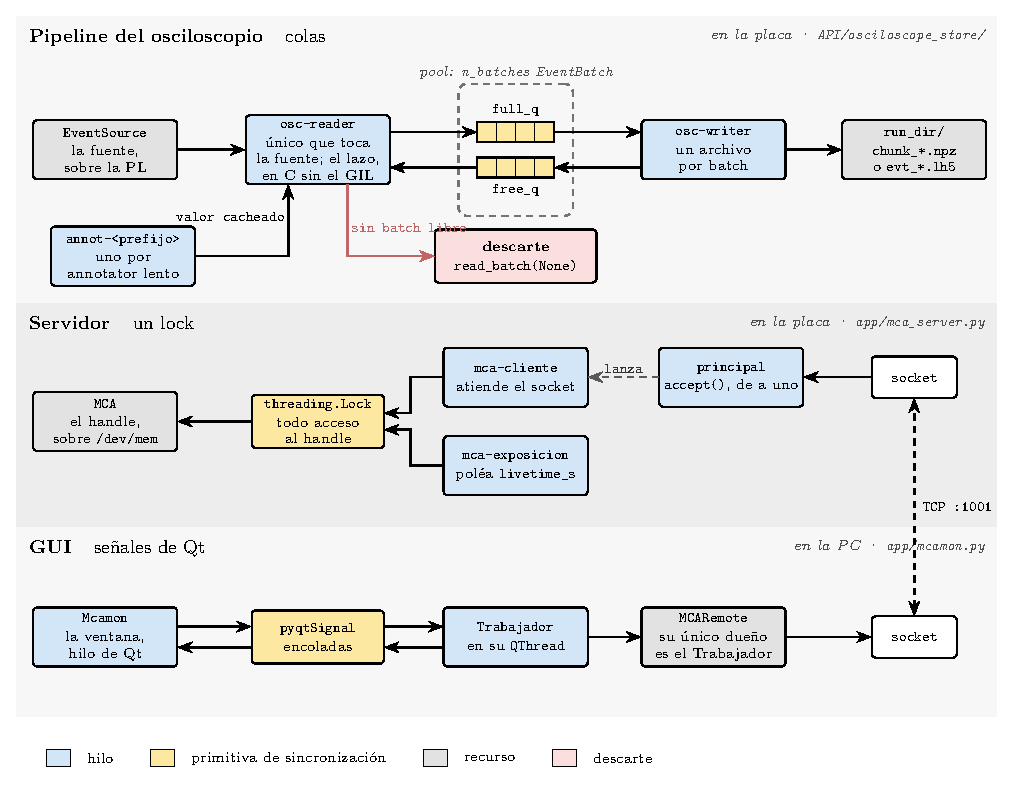
\includegraphics{cap10_hilos}
\caption[Las tres sesiones locales del programa]{%
Las tres sesiones locales de nuestro programa.\label{f:sw-hilos}}
\end{figure}

\begin{table}[H]
\centering
\caption[Hilos de captura y sus tareas]{%
Hilos de captura presentes en este proyecto y sus tareas
asociadas.\label{t:sw-hilos}}
\small
\begin{tabularx}{\textwidth}{|>{\raggedright\arraybackslash}p{0.19\textwidth}%
  |>{\raggedright\arraybackslash}p{0.22\textwidth}%
  |>{\raggedright\arraybackslash}X|}
\hline \encabezado \textbf{Hilo} & \textbf{Clase} & \textbf{Tareas} \\ \hline
principal & \codigo{AcquisitionSession} & arranca y detiene la adquisición;
  sólo espera (\codigo{wait}) y lee los contadores \\ \hline
\codigo{osc-reader} & \codigo{ReaderThread} & toma un \emph{batch} de
  \codigo{free\_q}, lo llena con \codigo{read\_batch}, les pide sus columnas a
  los anotadores y lo pasa a \codigo{full\_q} \\ \hline
\codigo{osc-writer} & \codigo{ChunkWriter} & toma un \emph{batch} de
  \codigo{full\_q}, lo guarda en un archivo y lo devuelve a \codigo{free\_q}
  \\ \hline
uno por anotador lento & \codigo{CachedAnnotator} & lee su sensor cada
  \codigo{interval\_s} y deja el valor en una caché \\ \hline
\end{tabularx}
\end{table}

El \codigo{osc-reader} no sabe de dónde vienen los eventos: lee de la fuente que
le den, \codigo{BramSource} o \codigo{RingSource}, y llena \emph{batches} de la clase
\codigo{EventBatch}. Cuando un \emph{batch} se llena (4096 eventos por defecto), lo
pasa a \codigo{full\_q}. El \codigo{osc-writer} guarda cada \emph{batch} que recibe,
así que queda un archivo por \emph{batch}: no hay un umbral de tamaño para escribir.

Los \emph{batches} son siempre los mismos objetos y circulan entre los dos hilos
(Fig.~\ref{f:sw-pool}). Al armar la sesión se crean entre 2 y 8, según el
presupuesto de RAM (\codigo{ram\_budget\_mb}, 64~MB por defecto), y después dan
la vuelta:
\begin{enumerate}
  \item \codigo{free\_q} le entrega uno al lector, que lo llena;
  \item El lector lo pone en \codigo{full\_q};
  \item El escritor lo toma y lo guarda;
  \item El escritor lo devuelve a \codigo{free\_q}.
\end{enumerate}
Es el esquema de productor y consumidor con un \emph{buffer}
acotado~\cite{Dijkstra1965}: \codigo{free\_q} y \codigo{full\_q} cuentan los
lugares vacíos y los llenos. Con los valores por defecto son 8 \emph{batches}, unos
5~MB en total. Los \emph{batches} llenos que esperan en \codigo{full\_q} son el margen
del escritor: a 10~kev/s puede atrasarse unos \qty{3}{\second} sin perder nada.
Si se atrasa más, \codigo{free\_q} se vacía y el lector descarta.

\begin{figure}[H]
\centering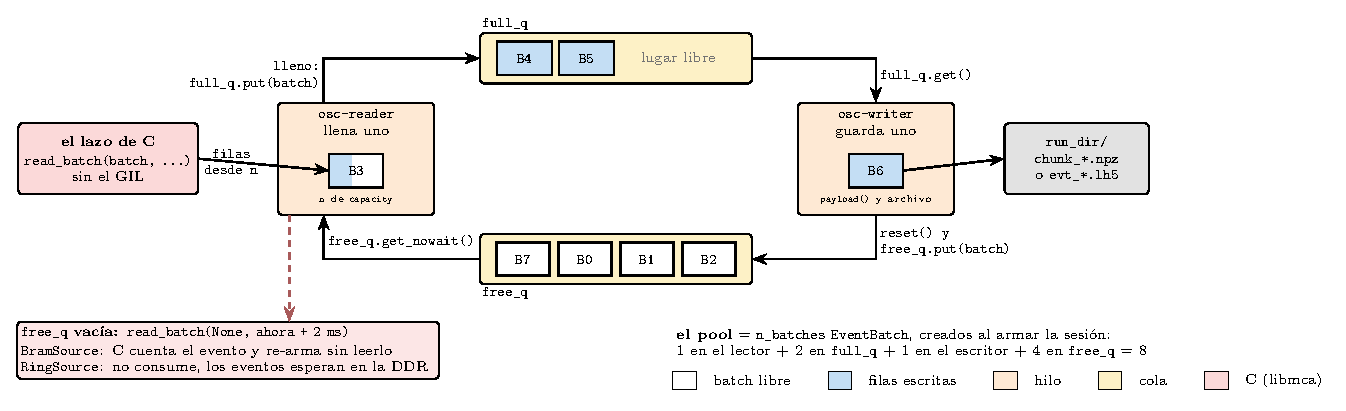
\includegraphics{cap10_pool_batches}
\caption[Cola de \codigo{EventBatch}]{%
Representación de la cola de \codigo{EventBatch}.\label{f:sw-pool}}
\end{figure}

En la Sec.~\ref{S:sw-flujo-sesion} describimos con más detalle cómo se inicia este sistema
mediante la utilización de la clase \codigo{AcquisitionSession}.

\subsubsection{Flujo de sesión de adquisición}
\label{S:sw-flujo-sesion}

En la Fig.~\ref{f:sw-flujo-sesion} se presenta el flujo de la sesión. Al
construirse, \codigo{AcquisitionSession} no toca el hardware ni lanza hilos:
arma el esquema del evento, crea los \emph{batches} del \emph{pool} y los pone en
\codigo{free\_q}. Para arrancar la medición (\codigo{start()}) sigue estos
pasos:
\begin{enumerate}
  \item Baja a \qty{1}{\milli\second} el intervalo de cambio del
    GIL~\cite{Beazley2010}, que por defecto es de \qty{5}{\milli\second}, para
    que el lector no espere tanto a que el escritor se lo devuelva.
  \item Arranca los anotadores. Los que leen sensores lentos lanzan su propio
    hilo.
  \item Arma la fuente (\codigo{source.arm()}): configura la PL, que queda
    esperando disparos.
  \item Arranca el hilo \codigo{osc-writer}, que queda esperando en
    \codigo{full\_q}.
  \item Arranca el hilo \codigo{osc-reader}, que empieza a llenar \emph{batches}.
\end{enumerate}

Mientras tanto, el hilo principal sólo espera (\codigo{wait()}): cada
\qty{0.2}{\second} revisa si se cumplió la duración o la cantidad de eventos, y
si se cayó un hilo o se llenó el disco.

Al finalizar (\codigo{stop()}), apaga en el orden inverso, para que no quede
ningún evento leído sin guardar:
\begin{enumerate}
  \item Con el ring, corta el estímulo con el hardware andando y espera, hasta
    \qty{5}{\second}, a que el lector se lleve lo que quedó en la DDR.
  \item Para el lector. Al salir, el lector pone en \codigo{full\_q} el \emph{batch}
    que tenía a medias y después un centinela (\codigo{None}).
  \item Espera al escritor, que guarda todo lo que hay en \codigo{full\_q} hasta
    encontrar el centinela.
  \item Para los anotadores, cierra la fuente (desarma la PL) y restaura el
    intervalo de cambio.
  \item Escribe \ruta{run_summary.json}, también con \ruta{.tmp} +
    \codigo{os.replace}.
\end{enumerate}

\begin{figure}[H]
\centering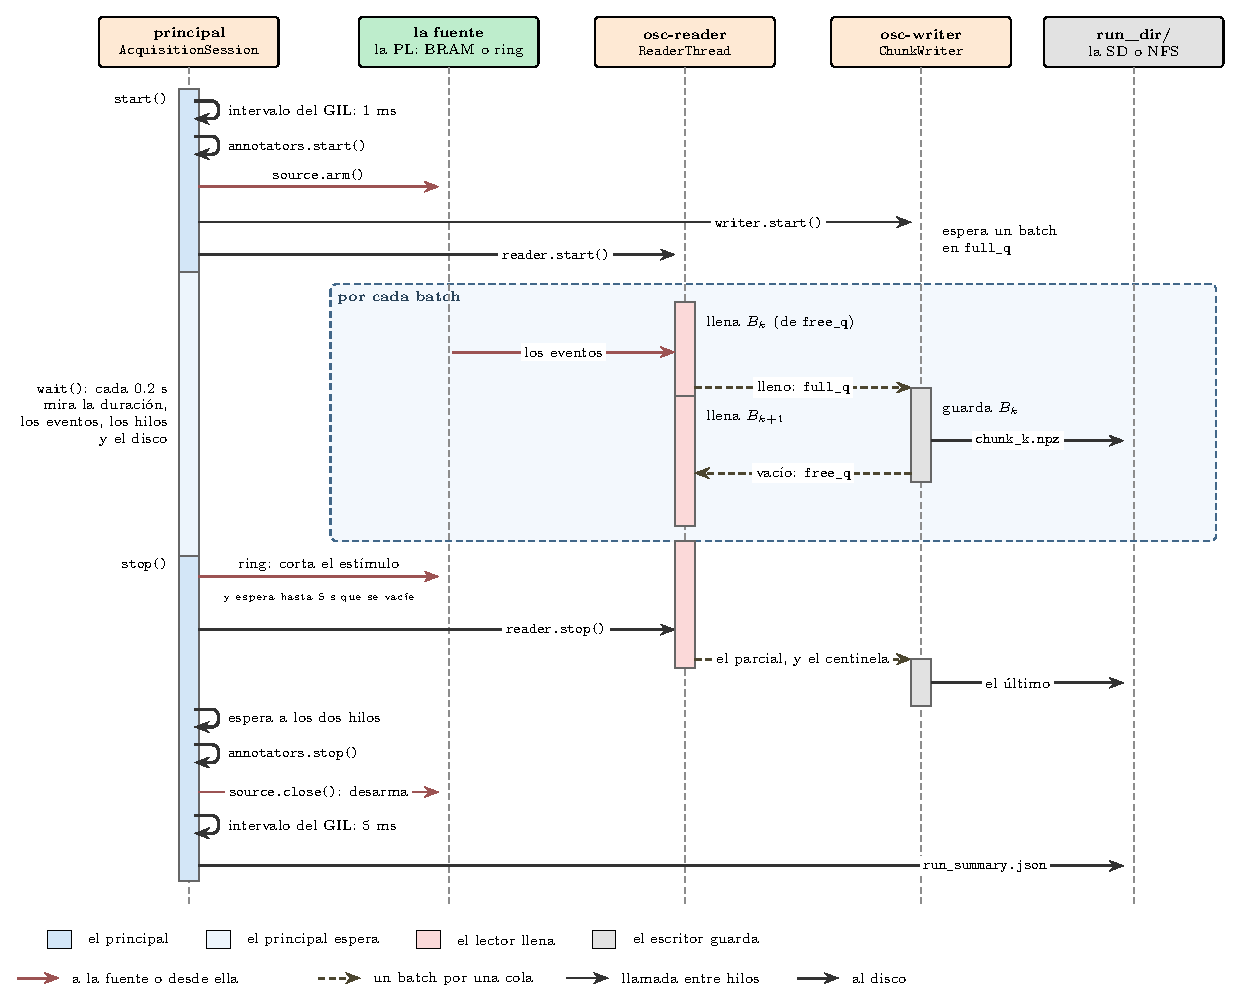
\includegraphics{cap10_flujo_sesion}
\caption[Flujo de trabajo de \codigo{AcquisitionSession}]{%
Flujo de trabajo del \codigo{AcquisitionSession}, de \codigo{start()} a
\codigo{stop()}. Por cada \emph{batch}, el lector lo llena con los eventos de la fuente
y lo pasa por \codigo{full\_q}, y el escritor lo guarda y lo devuelve por
\codigo{free\_q} mientras el lector ya llena el siguiente. Lo que pasa adentro de
cada hilo se presenta en la Fig.~\ref{f:ap-sw-hilos-captura}.\label{f:sw-flujo-sesion}}
\end{figure}

%==============================================================================
\section{Protocolo de red}
\label{S:sw-protocolo-red}

En el nivel de aplicación el sistema se comunica mediante mensajes \textbf{JSON
UTF-8 terminados en \codigo{\textbackslash n}}, seguidos opcionalmente de
\codigo{nbytes} crudos, en la Fig.~\ref{f:sw-trama}.

\begin{figure}[H]
\centering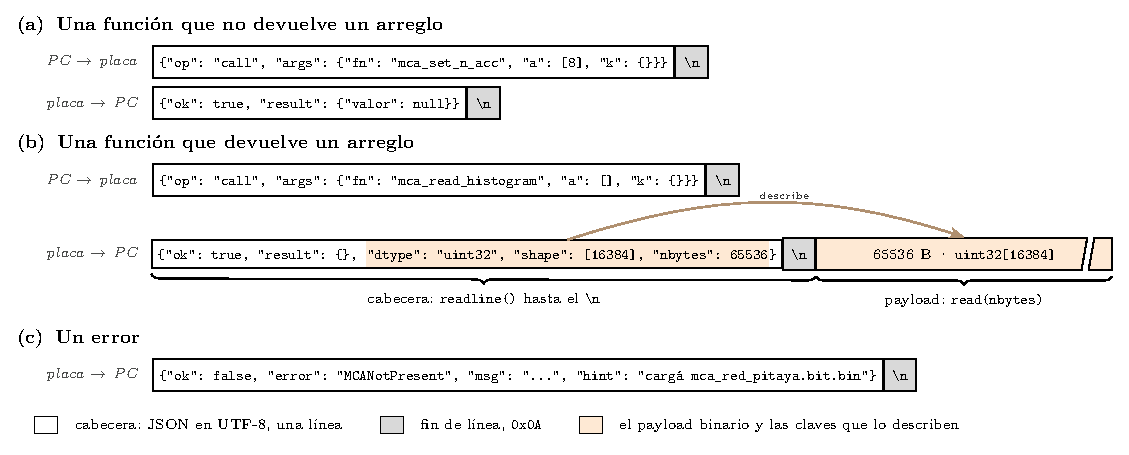
\includegraphics{cap10_trama}
\caption[Tramas del protocolo de red]{%
Ejemplos de tramas del protocolo de red: una cabecera JSON en una línea que
termina en \codigo{\textbackslash n} y el \emph{payload} binario que la cabecera
describe con \codigo{nbytes}, \codigo{dtype} y \codigo{shape}.
\label{f:sw-trama}}
\end{figure}

El flujo a nivel \emph{socket} está pensado para TCP: se creó una clase
\codigo{Channel} que tiene como objetivo serializar/deserializar la trama según
el protocolo. En la Fig.~\ref{f:sw-trama-flujo} se muestra la serialización
empleada en esta clase: mediante \codigo{readline()} obtiene fragmentos del
mensaje y mediante los \codigo{\textbackslash n} segmenta el mensaje.

\begin{figure}[H]
\centering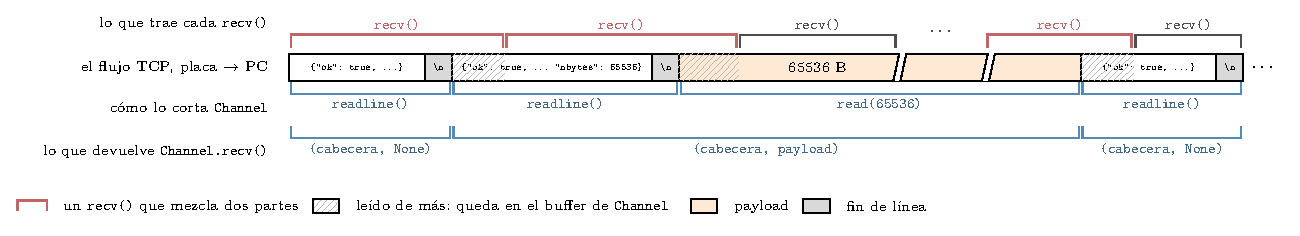
\includegraphics{cap10_trama_flujo}
\caption[Serialización de la trama en la clase \codigo{Channel}]{%
Serialización de trama JSON mediante la clase \codigo{Channel} empleando
\codigo{\textbackslash n}.\label{f:sw-trama-flujo}}
\end{figure}

\subsection{Modo de exportación de datos del ring}
\label{S:sw-exportacion-ring}

Los eventos del ring pueden llegar a un archivo por dos caminos, que se eligen
con el argumento \codigo{destino} de \codigo{ring.iniciar}. El primero es el de
la Sec.~\ref{S:sw-localizacion}: la sesión corre en la placa y escribe en una
dirección \codigo{run\_dir}, que puede estar en la microSD o en un disco de la
PC montado por NFS. Con NFS el archivo cruza la red, pero \textbf{lo sigue
armando la placa}. Eso resuelve la capacidad y la velocidad sostenida de la SD,
que limitan en corridas largas o con ventanas grandes, pero no saca del camino a
la sesión de Python en el procesador de la placa, que con ventanas cortas
también limita la tasa (Sec.~\ref{S:osc-ring-funcionamiento}).

El segundo, el modo de exportación por red, saca a la sesión del camino de los
datos en la placa (Fig.~\ref{f:sw-escritura-red}). No hizo falta una fuente
nueva: en este modo la placa no corre la sesión.

\begin{figure}[H]
\centering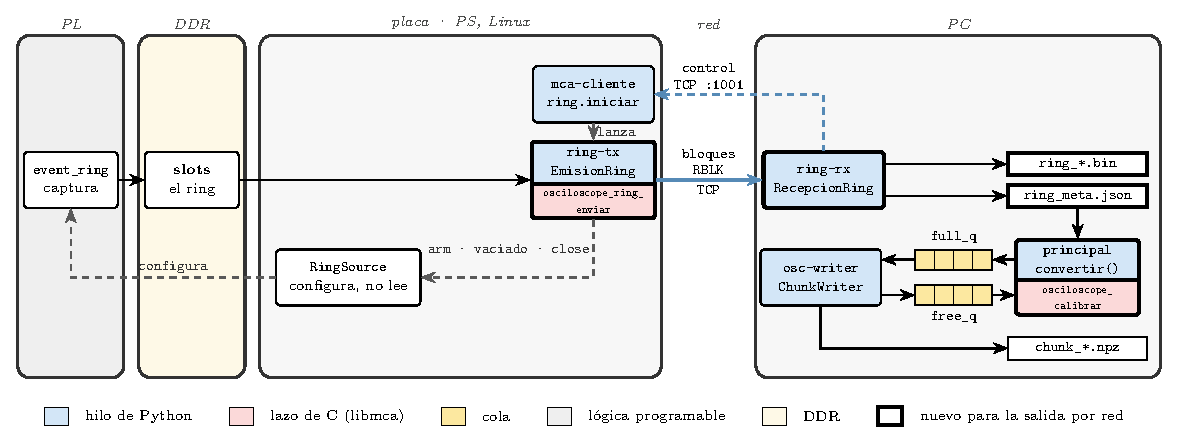
\includegraphics{cap10_escritura_archivos_por_red}
\caption[Escritura de los eventos del ring a archivos por red]{%
La escritura de los eventos del ring a archivos por red. En la placa no corre la
sesión: el hilo \codigo{ring-tx} llama a \codigo{osciloscope\_ring\_enviar}, que
copia los \emph{slots} y los manda en bloques \codigo{RBLK} por un \emph{socket} de datos, y
\codigo{RingSource} sólo configura el ring y el estímulo. En la PC,
\codigo{ring-rx} guarda el \emph{stream} tal cual en \ruta{ring_*.bin}, y
\codigo{convertir()} lo pasa a los mismos \ruta{chunk_*.npz} con el \emph{pool} y el
\codigo{ChunkWriter} de la sesión. El control va por el \emph{socket} del servidor (TCP
:1001).\label{f:sw-escritura-red}}
\end{figure}

Los datos y el control viajan por dos conexiones TCP distintas. El control usa
el \emph{socket} del servidor (TCP :1001) y el protocolo JSON de la
Sec.~\ref{S:sw-protocolo-red}. Después, la PC se conecta a ese puerto y recibe
un \emph{stream} de bloques con un formato propio. Cada bloque tiene una cabecera de
40~B (Tabla~\ref{t:sw-rblk}) y, detrás, \codigo{n} \emph{slots} tal como están en la
DDR: la cabecera del \emph{slot} (32~B) y las muestras int16 de los dos canales,
intercaladas y sin calibrar.

\begin{table}[H]
\centering
\caption[Cabecera de un bloque del \emph{stream} de datos]{%
Cabecera de un bloque del \emph{stream} de datos, en
\emph{little-endian}.\label{t:sw-rblk}}
\small
\begin{tabularx}{\textwidth}{|>{\raggedright\arraybackslash}p{0.3\textwidth}%
  |>{\raggedright\arraybackslash}p{0.2\textwidth}%
  |>{\raggedright\arraybackslash}X|}
\hline \encabezado \textbf{Campo} & \textbf{Tipo} & \textbf{Contenido} \\ \hline
\codigo{magic}, \codigo{version}, \codigo{flags} & u32, u16, u16 &
  \codigo{\textquotedbl RBLK\textquotedbl}, la versión 1 y el bit FIN \\ \hline
\codigo{seq0}, \codigo{n} & u32, u32 & el \codigo{seq} del primer \emph{slot} y la
  cantidad de \emph{slots} \\ \hline
\codigo{carga}, \codigo{bytes} & u32, u32 & los bytes por \emph{slot} y los que siguen
  a la cabecera \\ \hline
\codigo{descartados} & u64 & los eventos descartados antes del primer \emph{slot} del
  bloque \\ \hline
\codigo{t\_ns} & i64 & el reloj de la placa al leer el bloque \\ \hline
\end{tabularx}
\end{table}

%==============================================================================
\section{Resultados de \emph{benchmark}}
\label{S:sw-bench}

Dividimos las mediciones en las dos secciones principales del SW: las de
\codigo{libmca} y las de guardado por sesión en Python.

\subsection{Resultados de \emph{benchmark} para \texorpdfstring{\texttt{libmca}}{libmca}}
\label{S:sw-bench-libmca}

Se midió la misma operación por tres caminos, con el resultado de la
Tabla~\ref{t:sw-bench-libmca}:
\begin{itemize}
  \item \textbf{Python sin \emph{binding}}: la referencia, que lee los registros con
    \codigo{struct.unpack\_from} sobre el mmap, sin pasar por C;
  \item \textbf{Python con \emph{binding}}: Python $\rightarrow$ \codigo{ctypes}
    $\rightarrow$ \codigo{libmca};
  \item \textbf{C puro}: la misma función de \codigo{libmca}, llamada desde un
    programa en C sin intérprete.
\end{itemize}

\begin{table}[H]
\centering
\caption[Costo de llamada de las operaciones de \codigo{libmca}]{%
Tabla comparativa de costo de llamada de operaciones.\label{t:sw-bench-libmca}}
\begin{tabular}{|l|r|r|r|}
\hline \encabezado \textbf{Operación} (\unit{\micro\second}) & \textbf{Python}
  & \textbf{\emph{binding}} & \textbf{C} \\ \hline
leer un registro (\codigo{r32}) & 10.5 & 56.8 & 1.5 \\ \hline
leer el umbral & 15.4 & 63.7 & 1.4 \\ \hline
escribir el umbral & 27.7 & 52.1 & 1.6 \\ \hline
identificar el bloque & 74.6 & 77.4 & 3.2 \\ \hline
leer los contadores & 269 & 215 & 10.7 \\ \hline
leer la configuración & 334 & 193 & 10.6 \\ \hline
configurar & 252 & 280 & 9.4 \\ \hline
leer el espectro (8192 canales) & 34\,264 & 1\,880 & 1\,700 \\ \hline
\end{tabular}
\end{table}

Con un solo registro, el \emph{binding} (\qty{56.8}{\micro\second}) es más lento que
Python sin \emph{binding} (\qty{10.5}{\micro\second}): casi todo es el costo fijo de
cruzar \codigo{ctypes} en cada llamada, no el bus. Como ese costo es por llamada
y no por dato, deja de importar cuando una llamada hace mucho trabajo. Leer el
espectro tarda \qty{34.3}{\milli\second} en Python y \qty{1.88}{\milli\second}
por el \emph{binding}: el \emph{binding} agrega apenas un \qty{10}{\percent} sobre C puro, y
casi todo el resto es el tiempo del bus (\qty{0.2}{\micro\second} por palabra).

\subsection{Guardado de archivos en disco}
\label{S:sw-bench-disco}

Medimos la escritura de archivos persistentes con el ring saturado, para trazas
de tres largos \codigo{pre+post}, por dos caminos: la sesión en la placa
guardando en su SD, y por red, donde el servidor manda los \emph{slots} y un cliente en
la PC arma los mismos \ruta{.npz}. En la SD, cada punto dura unos
\qty{22}{\second} y cuenta el \codigo{sync} del final, así que mide lo que llega
a la tarjeta y no al page \emph{cache}. Los resultados se presentan en la
Fig.~\ref{f:sw-bench-red}: (a) en eventos por segundo y (b) en MB/s. La red pasa
3.5, 3.3 y 2.2 veces más que la SD, en ese orden, de forma que concluimos que el
camino por red es significativamente más rápido, al costo de necesitar un
cliente externo. Sin embargo, íbamos a necesitar este cliente externo
igualmente, ya que la memoria secundaria de la placa se llenaría en cuestión de
minutos: a 15~MB/s, los 1.4~GB libres duran un minuto y medio.

\begin{figure}[H]
\centering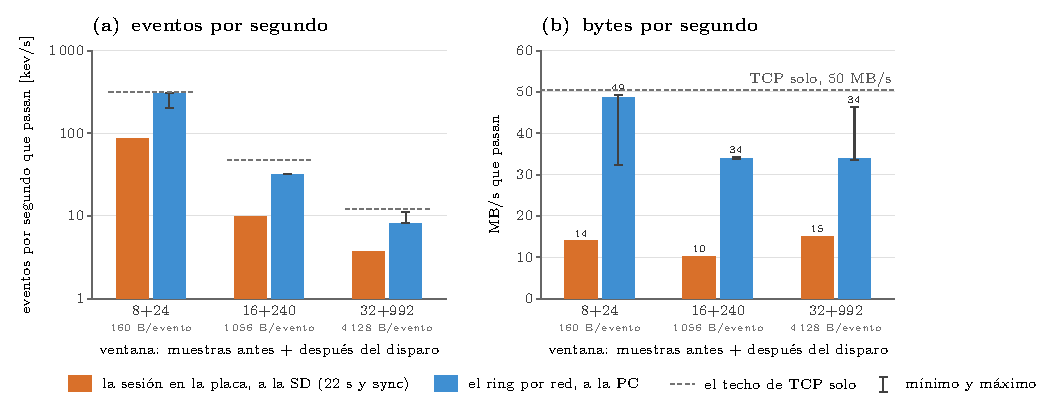
\includegraphics{cap10_bench_sd_red}
\caption[\emph{Benchmark} de escritura de archivos en la SD y por red]{%
\emph{Benchmark} de escritura de archivos. (a) En eventos por segundo, en escala
logarítmica; la raya es el techo de TCP sólo para ese tamaño de evento. (b) En
MB/s.\label{f:sw-bench-red}}
\end{figure}

% Bibliografía de este capítulo. Va al final del archivo, siempre.
\bibliografiacapitulo

%%% Local Variables:
%%% mode: latex
%%% TeX-master: "template"
%%% End:
